\chapter{\drexmtitle: multiple mantle aggregates LPO fabrics with D-Rex}
\label{chapter:drexm}

\drexmtitle{} is a software that computes the evolution of the LPO and related elastic properties of multiple mantle aggregates, as a function of the flow field, deformation mechanisms and P-T conditions given by large-scale geodynamic simulations, and of the single crystal plastic and elastic properties. It builds on the original \textbf{D-Rex} software \citep{kaminski2004gji}.\\
\\
The original \textbf{D-Rex} code estimates the strain-induced LPO of upper mantle polycrystalline aggregates in 2D assuming steady-state flow and that the whole deformation is accommodated by dislocation creep \citep{kaminski2004gji}.\\*
\drexmtitle{} additionally accounts for:
\begin{itemize}
    \item non steady-state flows in 2D/3D cartesian/polar grids \citep{faccenda2013g3,hu2017EPSL}. The fabrics for global-scale simulations are computed using the Yin-Yang grids (\citet{kageyama2004g3});
    
    \item fabrics within the mid and lowermost mantle, including those for post-Perovskite. Phase transitions can be set to occur at defined depths (e.g., 410 km, 660 km), density crossovers (which allows modeling the deflection of phase boundaries with a non-null Clapeyron-slope), and parameterized phase boundary as for the case of Brd -> pPv \citep{oganov2004nature};  
    
    \item elastic properties scaled by local P-T conditions \citep{faccenda2014pepi,chang2016natcomm,ferreira2019natgeo}. The isotropic component of the elastic tensors is taken from the lookup tables generated with \mmaeostitle{} for different lithologies, while the anisotropic component from the pressure and temperature derivatives of the single crystal elastic moduli. This strategy ensures a gradual transition of the elastic properties at phase boundaries where mineral aggregate transformation occurs;
    
    \item fabric evolution in presence of multiple creep mechanisms. Only the fraction of deformation accommodated by dislocation creep is used for intracrystalline deformation, while the remaining for rigid body rotation (e.g., \citep{hedjazian2017EPSL});
    
    \item imposing a pre-existing (fossil) fabric (pre-computed with \drexstitle{}) within a subdomain, typically the lithosphere. This is often the case for geodynamic models where the lithosphere accretion is not modeled, and its geometry is initially prescribed;
    
    \item extrinsic elastic anisotropy \citep{faccenda2014pepi,sturgeon2019g3} which can be superimposed over the LPO fabrics during visualization of the output with \viztomotitle{} (see section \textbf{\ref{section:elasticSPO}}).
    
    \item parallelization of its routines using a hybrid MPI and OpenMP scheme.

\end{itemize}
\vspace{0.5cm}
\texttt{COMPILE: ./bash\_compile}\\*

\texttt{RUN: mpirun -np nprocs ./drexm drexm\_input.dat}\\*

\section{Software structure and modus operandi}
\drexmtitle{} is structured as the following:
\begin{enumerate}
    \item the \drexmtitle{} model parameters are loaded from \texttt{drexm\_input.dat}, and the Eulerian grid (where the Eulerian fields are defined) and Lagrangian grid (mantle aggregates distribution) initialized accordingly. 
    \item the \textbf{V} (velocity), \textbf{P} (pressure), \textbf{Tk} (temperature), \textbf{Fd} (fraction of deformation accommodated by dislocation creep) Eulerian fields of the geodynamic model are loaded from the input \vtptitle{} files. 
    \item firstly, the mantle aggregates are advected backward in time for a desired time span (note that is different from the original D-Rex where the particles are advected backward in time for a desired amount of strain).
    \item successively, the mantle aggregates are advected forward and the strain-induced LPO and F\textsubscript{ij} evolution are simultaneously calculated. The forward run status can be checked in \texttt{cycle.txt} displaying the processed \vtptitle{} file number and the terminated iterations/cycles.  
    \item output \cijkltitle{} files are generated containing, among other infos, the elastic tensor \textbf{C}, density and the deformation gradient tensor \textbf{F} of each aggregate. 
\end{enumerate}

\section{Coordinate systems}
The coordinate system of the \drexmtitle{} computational domain is defined by axis 1, axis 2 and, in 3D, axis 3.\\
In cartesian coordinates, axis 1 is the horizontal direction, axis 2 depth, and, in 3D, axis 3 is the second horizontal direction.\\
In polar coordinates, axis 1 is longitude (in degrees), axis 2 the radial distance, and in 3D, axis 3 is colatitude (in degrees).\\
The vertical axis 2 can be positive either upward or downward.

\section{Input \vtptitle{} files}
In order to perform the operations mentioned in the previous section, input files named \vtptitle{}, where * is the file number, must be provided containing information about the geodynamic model evolution.

Essential information the input \vtptitle{} files should contain is:
\begin{itemize}
    \item the total elapsed time \fonts{timesum} and the timestep \fonts{dt} (time interval over which the fields are representative; normally it is the difference with the total elapsed time of the previous input \vtptitle{} file, if any. See section \ref{section:often}) of the geodynamic model as a HDF5 attribute \texttt{/Time}.
    \item the components of the Eulerian velocity vector field \textbf{V} saved in \texttt{/Nodes/V1}, \texttt{/Nodes/V2}, and in 3D, \texttt{/Nodes/V3}.
\end{itemize}

In addition, the following Eulerian fields can be provided:
\begin{itemize}
    \item when the geodynamic model is thermo-mechanical, the temperature \textbf{Tk} and total pressure \textbf{P} fields saved in \texttt{/Nodes/Tk} and \texttt{/Nodes/P}. These fields will be used to compute the elastic tensors as a function of the local P-T conditions.
    \item when the rheological model is based on multiple visco-plastic deformation mechanisms, the fraction of deformation accommodated by dislocation creep saved in \texttt{/Nodes/Fd}, where \textbf{Fd} = $nu_{disl}/nu_{eff}$, 0 $\leq$ \textbf{Fd} $\leq$ 1, $nu_{disl}$ is the viscosity calculated with the dislocation creep flow law, $nu_{eff}$ is the effective viscosity which is typically calculated with the harmonic average of each of the viscosities representing a different deformation mechanism. 
\end{itemize}

Summarizing, the time infos and the velocity field are essential, while the other 3 fields are optional and depend on the type of (mechanical vs. thermomechanical) geodynamic and (single vs. multiple visco-plastic deformation mechanisms) rheological models.

\subsection{How saving information from your geodynamic model?}
Examples of how to build the input file in HDF5 format with \matlabtitle{} are provided in directory \texttt{/D-REX\_M/make\_HDF5\_vtp\_files}.

\textbf{Indexing}: since the \textbf{V}, \textbf{P}, \textbf{Tk}, \textbf{Fd} Eulerian fields are loaded as 1D HDF5 datasets, they must be provided as 1D arrays where the nodes are indexed going through the grid axes sequenced as:
2D models: axis 2, axis 1. That is, Y, X axes in cartesian coordinates, and Radial, Long. axes in polar coordinates.
3D models: axis 2, axis 1, axis 3. That is, Y, X, Z axes in cartesian coordinates, and  Radial, Long., Colat. axes in spherical coordinates. 

\textbf{Units}: values in attribute \texttt{/Time} and \textbf{V} as well as those of variables (i.e., \fonts{timemax} or distances) in the input file \texttt{drexm\_input.dat} should be provided using consistent units for time and length, and which can be of any type (e.g., dimensional (i.e., [cm,yr] or [m,s]) or adimensional). In contrast, the \textbf{P} and \textbf{Tk} Eulerian fields must always be in Pa and K.

The Eulerian fields of the geodynamic model must be defined on the same node positions of the Eulerian grid defined in \texttt{drexm\_input.dat}. The Eulerian grid must be regular (i.e., same node spacing along a given axis; if other types of grid are required, please contact the software developer).\\
For 3D global-scale simulations, the Yin-Yang Eulerian grids \citep{kageyama2004g3} are used to ensure a more homogeneous sampling of the spherical domain (see section \ref{section:cookbook_3Dspherical_global}).\\ 
In cartesian coordinates, the velocity field can also be defined on staggered additional nodes, which allows to compute the velocity gradient tensor with a numerical resolution that is double than when the velocity vector components are all defined on the same basic node.  
In 2D, V1 is shifted by $+\Delta x_2/2$ and V2 by $+\Delta x_1/2$ with respect to the basic node. 
In 3D, V1 is shifted by $+\Delta x_2/2$ and $+\Delta x_3/2$, V2 by $+\Delta x_1/2$ and $+\Delta x_3/2$, V3 by $+\Delta x_1/2$ and $+\Delta x_2/2$ with respect to the basic node.

\subsection{How often saving information from your geodynamic model?}
\label{section:often}
\textbf{Time-dependent flows}: From our experience, for Earth-like deformation rates it is sufficient to save the \textbf{V}, \textbf{P}, \textbf{Tk} and \textbf{Fd} fields averaged every 100/200 kyr, a time span over which these fields do not vary substantially. This will prevent outputting too many files from the geodynamic model. The code will then calculate an advection timestep which fulfill the Courant criterion and iterate for several cycles upon reaching the timestep defined in \texttt{/Time}.\\

\textbf{Steady-state flows}: in this case, it is clear that only a single \vtptitle{} file is needed.

\subsection{Which is the model time interval over which \drexmtitle{} should run?}
\citep{boneh2014epsl} showed that a cumulative strain of 5 is sufficient to reset any previous LPO and develop a new one. This is indeed the maximum cumulative strain that the original \textbf{D-Rex} consider for LPO calculation of each mantle aggregate.
For typical mantle deformation rates of $10^{-15}-10^{-14}    s^{-1}$, this amount of deformation is acquired in about  3 – 30 Myr. This is the model time interval during which input \vtptitle{} files must be saved in your time-dependent geodynamic model. Thus, saving an input \vtptitle{} file every 200 kyr over a time span of 20 Myr, implies saving and processing 100 input files.\\
There exist cases where the model time interval could be larger, such as when it is desired to model the fabrics forming at oceanic ridges and successively advected for several tens of Myr within the rigid lithosphere till the subduction zone. However, steady-state corner flow is often assumed for this particular set of models, which implies that only a single \vtptitle{} file is needed.

\section{Output \cijkltitle{} files}
Output files includes, for each aggregate, its rocktype, position, density, elastic tensor \textbf{C} and deformation gradient tensor \textbf{F}. When available, the aggregate P-T conditions are additionally saved.
The \textbf{C} tensor is calculated as a function of the crystals orientation, volume fraction, modal composition of the aggregate (e.g., 70:30=Ol:Ens in hartzburgitic mantle), single crystal elastic properties scaled by the local P-T conditions, and with a Reuss-Voigt averaging scheme.\\
An output \cijkltitle{} file is always generated at the end of the simulation, whereby the aggregates, after the backward and forward advection episodes, display the same initial (regular) distribution. Output files at intermediate steps can be generated by setting \fonts{OutputStep} smaller than the total number of computing cycles of the forward advection scheme, with the characteristic that the aggregate distribution will be irregular. 

\section{Allocated memory}
Memory is allocated in large part to track the mineral aggregates properties and, to a minor extent, for storing the loaded the Eulerian node fields. Thus in case of 100s of thousands or millions of aggregates, problems related to insufficient memory allocation may occur.\\
For a 3D model, the memory allocated for the Eulerian fields is up to $24*8$ bytes per node. Thus, around 200 MB of memory is necessary every 1 million nodes per each MPI process.\\
For each mineral aggregates, the allocated memory is up to $(75 + 20*\fonts{size3})*8$ bytes, thus very sensitive to the number of crystals. When $\fonts{size3}=8$, there are $512*2$ crystals per aggregate, and thus 82.5 kB per aggregate. Hence, over 80 GB of memory is necessary every 1 million aggregates.

\section{Parameter input file}
\label{section:modelsetup}

The following information need to be set in the parameter  input file \texttt{drexm\_input.dat} (unless otherwise specified, the variable format is \texttt{double precision}):

MPI proc distribution along axis
\begin{itemize}
    \item \fonts{nproc1}, \fonts{nproc2}, \fonts{nproc2}: (Integer) number of MPI subdomains (processes) along axes 1, 2 and 3
\end{itemize}
(WARNING: the number of MPI processes \fonts{nproc1}*\fonts{nproc2}*\fonts{nproc3} must be > 1)
\vspace{1cm}

A) Input and output directories/files
\begin{itemize}
    \item \fonts{input\_dir}: (String) path to the input \vtptitle{} files directory (the path should end with  “/” )
    \item \fonts{output\_dir}: (String) path to the directory where the output \cijkltitle{} file is saved (the path should end with  “/” )
    \item \fonts{Tinit, Tstep, Tend}: (Integers) initial, increment and final number of input \vtptitle{} files. Set \fonts{Tinit} = \fonts{Tend} for steady-state models. 
    \item \fonts{OutputStep}: (Integer) number of cycles interval after which an output file is generated during forward advection.
    \item \fonts{timemax}: time span (in Myr for dimensional time) for steady-state models
\end{itemize}
\vspace{1cm}

B) Define the computational domain:
\begin{itemize}
    \item \fonts{dimensions}: (Integer)
        \begin{itemize}
         \item[] \fonts{2} = 2D model
         \item[] \fonts{3} = 3D model
        \end{itemize}
    \item \fonts{cartspher}:  (Integer) 
        \begin{itemize}
         \item[] \fonts{1} = cartesian coordinate system
         \item[] \fonts{2} = polar coordinate system
        \end{itemize}
    \item \fonts{basicstag}: velocity field defined on:  (Integer) 
        \begin{itemize}
         \item[] \fonts{1} = basic nodes
         \item[] \fonts{2} = staggered nodes\footnotemark
    \end{itemize}
\end{itemize}

\vspace{0.2cm}

Eulerian grid (i.e., where the \textbf{V}, \textbf{P} and \textbf{Tk} fields are defined):
\begin{itemize}

    \item \fonts{x1min}, \fonts{x1max}, \fonts{nx1}, \fonts{x1periodic}: define Eulerian axis 1: min, max coordinates (in unit length in cartesian coord.; in degrees in polar/spherical coord.), number of nodes (Integer), periodic (\fonts{1}) or not (\fonts{0}) (Integer).  
    \item \fonts{x2min}, \fonts{x2max}, \fonts{nx2}, \fonts{x2periodic}: define Eulerian axis 2: min, max coordinates (in unit length), number of nodes (Integer), periodic (\fonts{1}) or not (\fonts{0}) (Integer).  
    \item \fonts{x3min}, \fonts{x3max}, \fonts{nx3}, \fonts{x3periodic}: define Eulerian axis 3: min, max coordinates (in unit length in cartesian coord.; in degrees in spherical coord.), number of nodes (Integer), periodic (\fonts{1}) or not (\fonts{0}) (Integer).  
\end{itemize}

\vspace{0.2cm}
Lagrangian grid (i.e., the initial and final position of the mantle aggregates):
 
\begin{itemize}   
    \item \fonts{mx1min}, \fonts{mx1max}, \fonts{mx1stp}: define particle distribution along axis 1: min, max coordinates (in unit length in cartesian coord.; in degrees in polar/spherical coord.), spacing (in unit length, also for polar coordinate system)
    \item \fonts{mx2min}, \fonts{mx2max}, \fonts{mx2stp}: define particle distribution along axis 2: min, max coordinates, spacing (in unit length)
    \item \fonts{mx3min}, \fonts{mx3max}, \fonts{mx3stp}: define particle distribution along axis3: min, max coordinates (in unit length in cartesian coord.; in degrees in spherical coord.), spacing (in unit length, also for polar coordinate system)
\end{itemize}
\vspace{1cm}

\footnotetext{The staggered nodes can be defined only for cartesian grids}


C) LPO parameters:
\begin{itemize}
    \item \fonts{size3}\footnotemark: (Integer) cubic root of total number of grains in the aggregate for each of the 2 mineral phases (e.g.: \fonts{size3} = 10 $\rightarrow$ 1000 crystals of phase 1 and 1000 crystals of phase 2). 
\end{itemize}
\vspace{0.5cm}

\footnotetext{The size of the allocated memory is mostly sensitive to this parameter, be careful!}

    For each of the 5 different rocktype (Ol:Ens; Wd:Grt; Rw:Grt\footnotemark; Brd:MgO; pPv:MgO\footnotemark):
\begin{itemize}
    \item \fonts{Xol}: volume fraction of Ol, Wd, Rw, Brd, pPv (in \%)
    \item \fonts{minx2,maxx2}: min, max vertical distribution (in unit length)
    \item \fonts{stressexp}: stress exponent for non-Newtonian plasticity  
    \item \fonts{Mob}: efficiency of grain boundary migration 
    \item \fonts{chi ($\pmb{\chi}$)}: volume fraction threshold below which no dislocation creep occurs   
    \item \fonts{lambda ($\pmb{\lambda}$)}: efficiency of grain nucleation
    \item \fonts{fractdislrock}: fraction of deformation accommodated by the anisotropic phase. It assumes values between 0.0 (no deformation) and 1.0 (all deformation accommodated by the anisotropic phase). It should be always 1.0 for UM aggregates where both olivine and enstatite are anisotropic.
    \item \fonts{tau1...tauN}: normalized CRSS of the anisotropic phase slip systems. For upper mantle aggregates, one additional tau5=1 is added for enstatite. See \ref{table:1}.
    \item \fonts{single\_crystal\_elastic\_db}: (Integer) choose single crystal elastic tensor for phase 1 and 2 from those compiled in \texttt{elastic\_database.f90}. See \ref{table:2}.
\end{itemize}

\footnotetext{Rw and Grt are considered as isotropic at MTZ, and therefore only \textbf{Xol,minx2,maxx2} and \textbf{single\_crystal\_elastic\_db} need to be set}
\footnotetext{the occurrence of pPv is set according to the parametrized phase boundary by \citet{oganovono2004nature}, and therefore \textbf{minx2,maxx2} should not be set. Hence, \fonts{ptmod} = 2}

\vspace{1cm}

D) Pre-existing (fossil) fabric. The fabric (given by the LPO and \textbf{F}) computed for a single aggregate in directory \texttt{/D-REX\_S} is assigned to all aggregates within a given subdomain defined below:
\begin{itemize}
    \item \fonts{fossilfabric}: (Integer)
    \begin{itemize}
        \item[] \fonts{0} = no pre-existing fabric 
        \item[] \fonts{1} = the pre-existing fabric is set after backward advection and before computing the LPOs 
        \item[] \fonts{2} = the pre-existing fabric is set at the end of the model replacing the computed LPOs
    \end{itemize}
    \item \fonts{mx1minfab}, \fonts{mx1maxfab}: distribution of aggregates with pre-existing fabric along axis 1 (in unit length in cartesian coord.; in degrees in polar/spherical coord.)
    \item \fonts{mx2minfab}, \fonts{mx2maxfab}: distribution of aggregates with pre-existing fabric along axis 2 (in unit length)
    \item \fonts{mx3minfab}, \fonts{mx3maxfab}: distribution of aggregates with pre-existing fabric along axis 3 (in unit length in cartesian coord.; in degrees in spherical coord.)
\end{itemize}
In polar coordinates, the loaded LPO and \textbf{F} are rotated according to the aggregate longitude and colatitude. Thus, when computing the single aggregate fabric with \texttt{/D-REX\_S}, bear in mind that axis 1, 2 and 3 should correspond to longitude, depth and colatitude, respectively. 
\vspace{1cm}

E) Operating modes:
\begin{itemize}

    \item \fonts{fsemod}: (Integer)
    \begin{itemize}
        \item[] \fonts{0} = compute strain-induced \textbf{F} and LPO evolution
        \item[] \fonts{1} = compute only \textbf{F} evolution, and \fonts{fractdislmod}, \fonts{fabrictransformmod} and \fonts{ptmod} are set to 0.
    \end{itemize}
    
    \item \fonts{uppermantlemod}: (Integer)
    \begin{itemize}
        \item[] \fonts{0} = \textbf{F}, LPO and advection for all aggregates.
        \item[] \fonts{1} = \textbf{F} and LPO only for upper mantle aggregates; advection for all aggregates. This mode is suggested when focusing on UM anisotropy only. The elastic tensor of deeper mantle aggregates are computed assuming isotropy. As a consequence, the execution of the run is much faster.
    \end{itemize}
    
    \item \fonts{fractdislmod}: (Integer)
    \begin{itemize}
        \item[] \fonts{0} = 100\% of the deformation is accommodated by dislocation creep. 
        \item[] \fonts{1} = use only fraction of deformation accommodated by dislocation creep as interpolated from the \textbf{Fd} field. The \textbf{Fd} field need to be provided in input \vtptitle{} files.
    \end{itemize}
    
    \item \fonts{fabrictransformod}: (Integer)
    \begin{itemize}
        \item[] \fonts{0} = no phase transformation.
        \item[] \fonts{1} = retain LPO after phase transformation, simulating axisymmetric topotactic growth of the new phases.
        \item[] \fonts{2} = reset LPO after phase transformation
    \end{itemize}
    
    \item \fonts{ptmod}: (Integer)
    \begin{itemize}
        \item[] \fonts{0} = use single crystal tensors at room P-T conditions. Choose this when your geodynamic model is purely mechanical and there no is information about the local P-T conditions.
        \item[] \fonts{1} = scale elastic moduli and density by local P-T conditions, phase transitions occur at depths specified in top and bot; thus, the phase boundaries are horizontal. \textbf{Tk} and \textbf{P} fields need to be provided in input \vtptitle{} files.
        \item[] \fonts{2} = scale elastic moduli and density by local P-T conditions, phase transitions occurs at density crossovers (Ol+Ens $\leftrightarrows$ Wd+Grt at  3650 \si{kg/m^3}; Wd+Grt $\leftrightarrows$ Rw+Grt at  3870 \si{kg/m^3}; Rw+Grt $\leftrightarrows$ Brd+MgO at  4150 \si{kg/m^3}). This mode allows to model deflections of phase boundaries in proximity of mantle downwellings/upwellings. \textbf{Tk} and \textbf{P} fields need to be provided in input \vtptitle{} files.
    \end{itemize}
    
    The occurrence of pPv is determined with the parametrized phase transition by \citet{oganov2004nature}, thus \textbf{Tk} and \textbf{P} fields are necessary. In general, whenever the computational domain includes layers deeper than the upper mantle, \fonts{ptmod} > 0 is the preferred operational mode.
    
    In order to minimize the contrast in elastic properties among rocktypes and arising from contrasts in experimental single crystal elastic tensors and their P-T derivatives (see \ref{table:2}), the isotropic component of the aggregate elastic tensor is replaced with that computed with \mmaeostitle{} for a given lithology when \fonts{ptmod} > 0.
    
    \item \fonts{eosmod}: (Integer) set the domain lithology (\fonts{1}: Dunite; \fonts{2}: Harzburgite; \fonts{3}: Pyrolite; \fonts{4}: Basalt; \fonts{5}: Pyroxenite) for which the corresponding density, Vp and Vs lookup tables computed with \mmaeostitle{} are loaded (see Table \ref{table:3}).
    
    \item \fonts{fractvoigt}: fraction of Voigt averaging scheme when calculating the aggregate elastic tensor in \%. It varies from 0.0 (Reuss average) to 100.0 (Voigt average). When equal to 50.0\%, it yields the Hill average.
    
\end{itemize}

\section{Parallelization and its efficiency}
\drexmtitle{} routines are parallelized using a hybrid MPI and OpenMP scheme to take advantage of multi-CPU nodes and multicore architectures of modern HPC clusters. The parallel efficiency is close to 1 for most routines, with the update of the LPO and Fij tensor during the forward advection is the most time-consuming part of the run (Fig. \ref{fig:scalability}). The small performance degradation is due to the initialization of the Eulerian/Lagrangian grids and arrays, and to I/O operations (i.e., loading infos from input \vtptitle{} files, writing the output to \cijkltitle{})\\ which are executed serially within each process. As a result, the efficiency of the time-dependent flow models (such as the 3D sinking slab model) is lower than that of steady-state models (the 3D global flow model) because of the larger I/O operations ((i.e., loading infos from input \vtptitle{} files and compute the velocity gradient tensors, advection timestep, etc.).

\begin{figure}
    \centering
    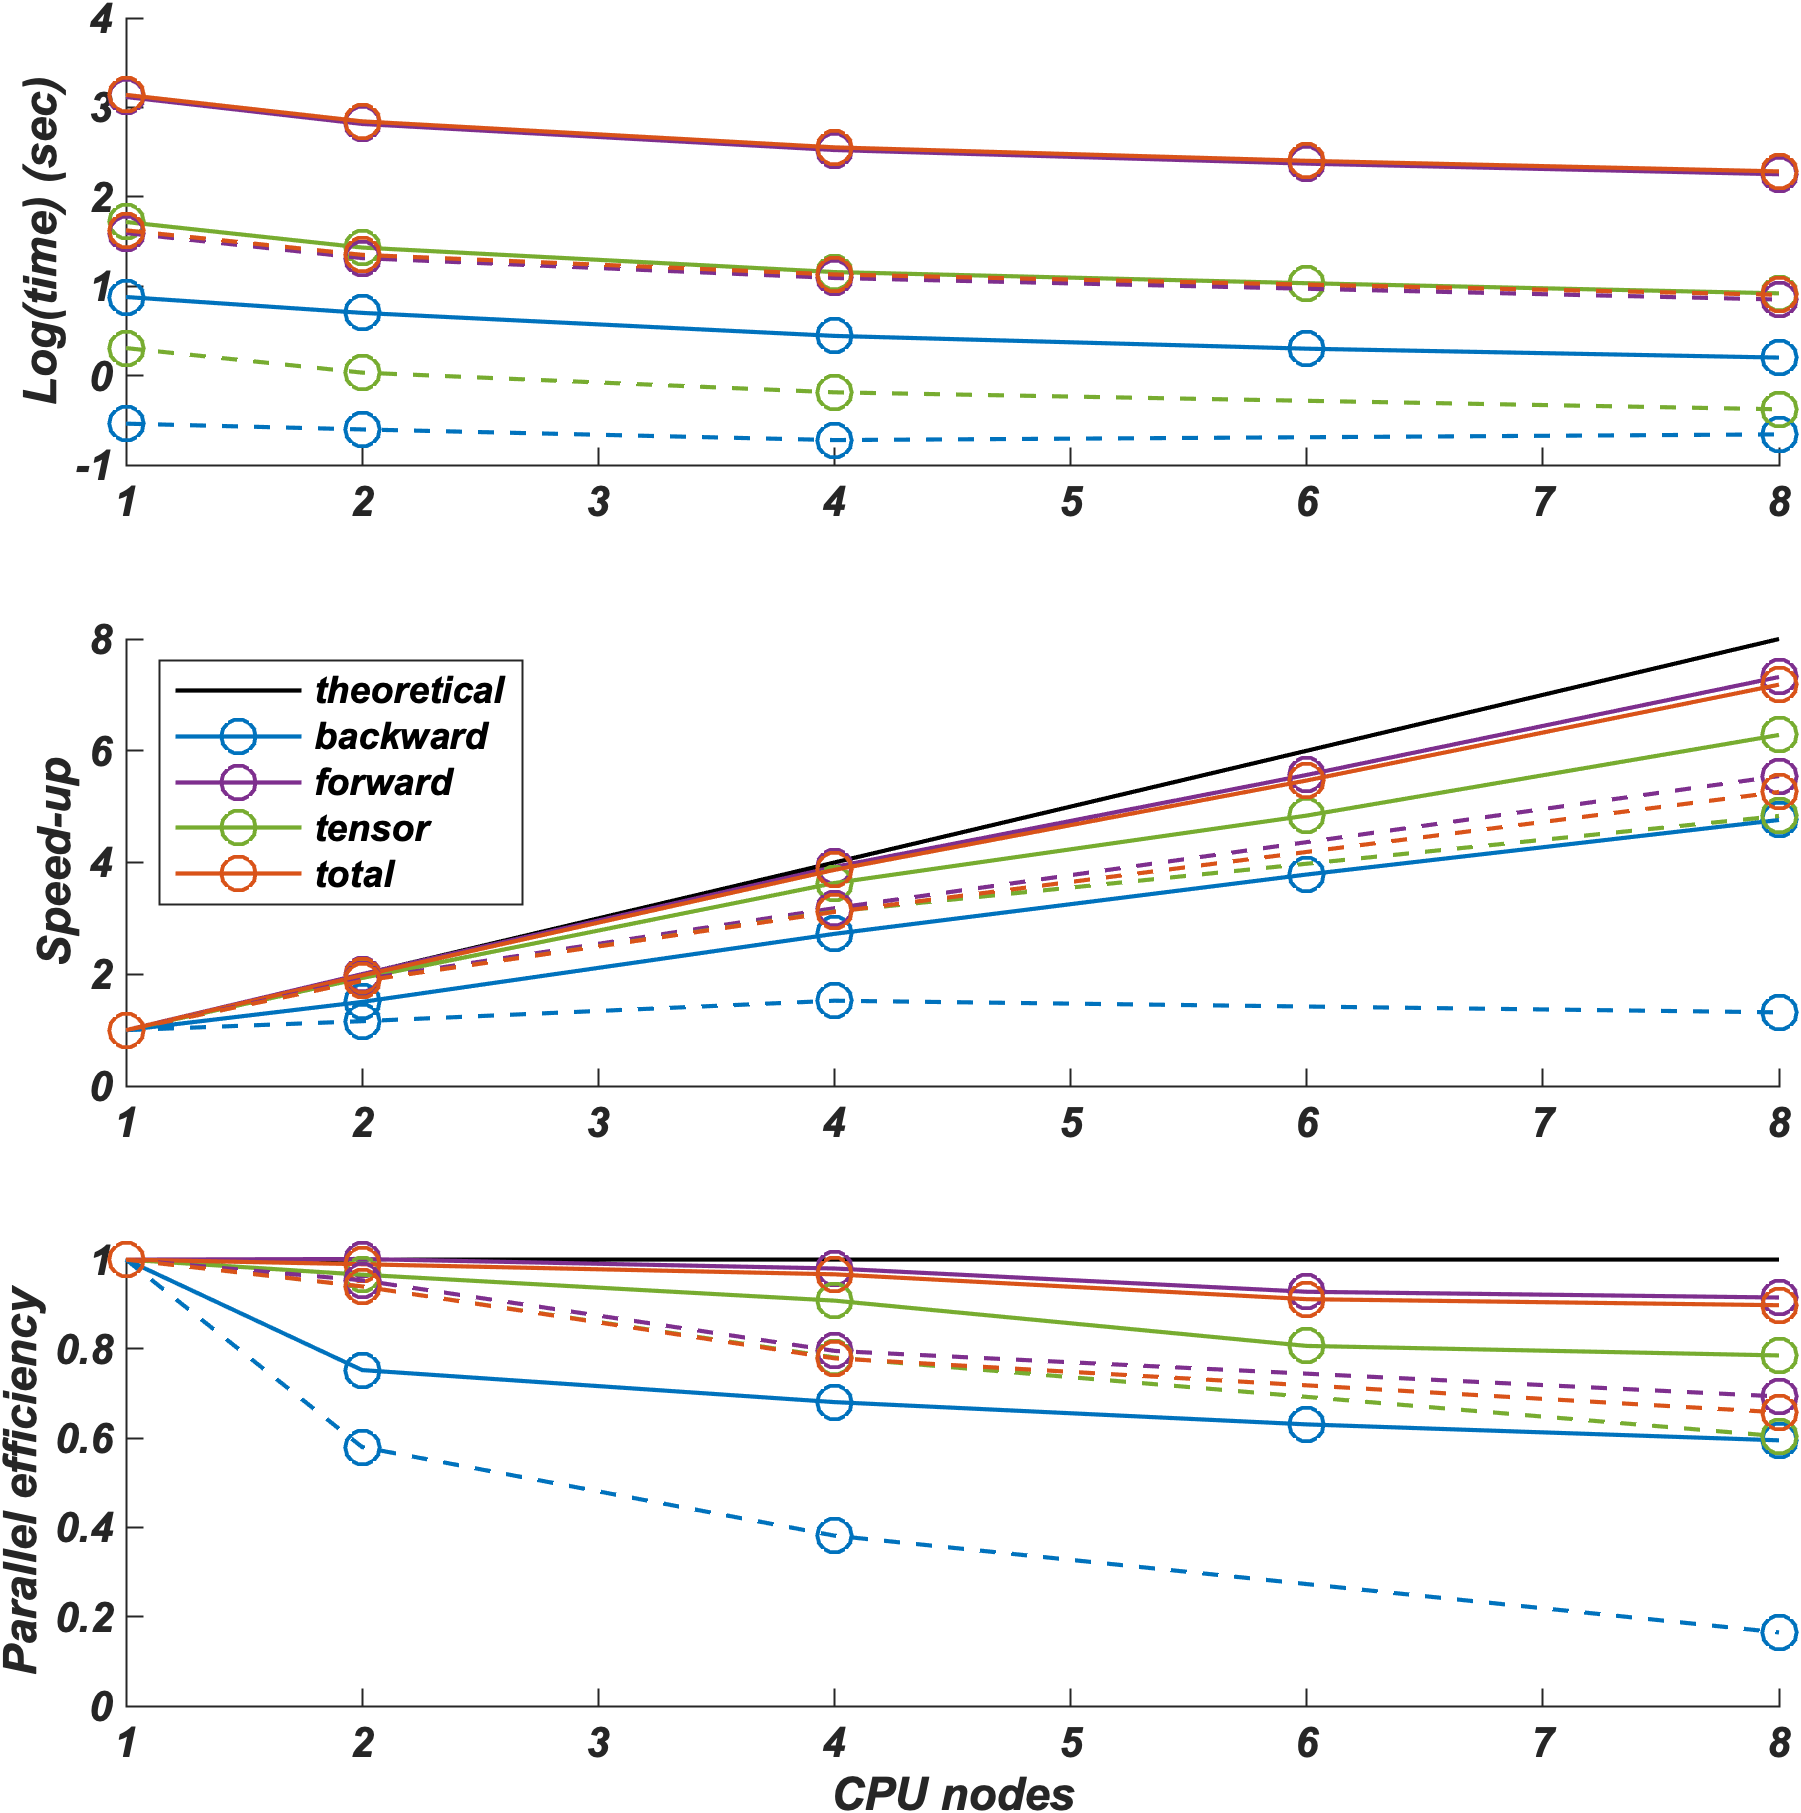
\includegraphics[width=0.8\textwidth]{DREX_M/drexm_time_speedup_scalability_log10.png}
    \caption{Runtime (top), speedup (centre) and parallel efficiency (bottom) of \drexmtitle{} for initial backward advection of aggregates (backward), forward advection and update of the LPO and Fij tensor (forward), full elastic tensor computation and output generation (tensor), and entire run (total). Results shown for two models included in the cookbooks: a 3D global convection model (steady-state flow, 96 timesteps, 1327606 aggregates, LPO computed only for 260474 upper mantle aggregates) and the 3D sinking slab model (dashed lines; time-dependent flow, 20 timesteps, 38509 aggregates, LPO computed for 25177 upper mantle and 6587 upper mantle transition zone aggregates). Runs performed on a HPE Superdome Flex (8 CPUs, 28 cores Intel Xeon(R) PLATINUM 8180 @ 2.50GHz) using from 1 to 8 nodes.
    }
    \label{fig:scalability}
\end{figure}

\vfill % Fill the rest of the page with whitespace